\documentclass{minimal}
\usepackage{tikz}
\usepackage[T1]{fontenc}

\usetikzlibrary{fadings}

\definecolor{boxbot}{RGB}{49,139,255}
\definecolor{boxtop}{RGB}{171,208,255}

\definecolor{normal}{RGB}{25,25,25}
\definecolor{keyword}{RGB}{196,0,5}
\definecolor{op}{RGB}{0,0,255}
\definecolor{number}{RGB}{0,0,120}
\definecolor{string}{RGB}{0,104,4}
\definecolor{ln}{RGB}{100,100,100}

\renewcommand\encodingdefault{T1}
\renewcommand\familydefault{fvm}

\newcounter{line}
\newcommand\resetlnr{\setcounter{line}{0}}
\newcommand{\lnr}{%
\stepcounter{line}%
\expandafter\ifnum\theline<10 ~\fi%
\textcolor{ln}{\theline}~~%
}

\newcommand\kw[1]{\textcolor{keyword}{#1}}
\newcommand\op[1]{\textcolor{op}{#1}}
\newcommand\val[1]{\textcolor{normal}{#1}}
\newcommand\num[1]{\textcolor{number}{#1}}
\newcommand\str[1]{\textcolor{string}{#1}}

\newcommand\ltag{\textcolor{op}{<\hbox{}<}}
\newcommand\rtag{\textcolor{op}{>\hbox{}>}}
\newcommand\sem{\textcolor{ln}{;}}

\begin{document}

\tikzstyle{every node}=[font=\normalfont]
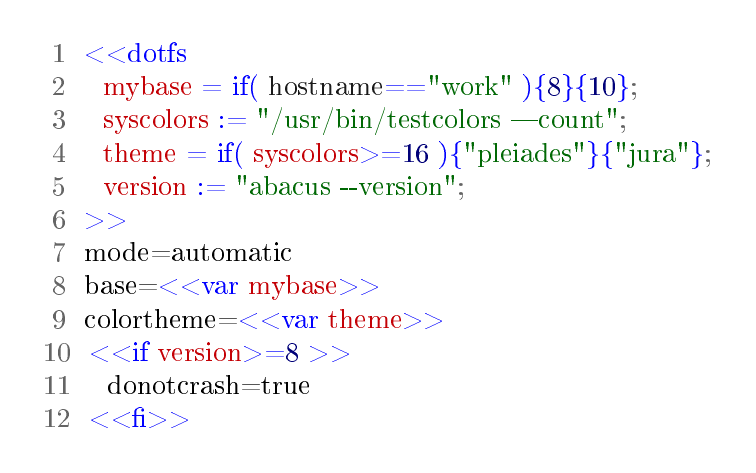
\begin{tikzpicture}[
box/.style={
	%bottom color=boxbot,
%    top color=boxtop,
    inner sep=2mm,
    rounded corners,
    align=left
},
normwidth/.style={
    minimum width=5cm,
    text width=5cm
}
]

\node[box] {\resetlnr
\lnr\ltag \op{dotfs}\\
\lnr~~\kw{mybase} \op= \op{if(} \val{hostname}\op{==}\str{"work"} \op{)\{}\num{8}\op{\}\{}\num{10}\op{\}}\sem\\
\lnr~~\kw{syscolors} \op{:=} \str{"/usr/bin/testcolors ---count"}\sem\\
\lnr~~\kw{theme} \op= \op{if(} \kw{syscolors}\op{>=}\num{16} \op{)\{}\str{"pleiades"}\op{\}\{}\str{"jura"}\op{\}}\sem\\
\lnr~~\kw{version} \op{:=} \str{"abacus -\hbox{}-version"}\sem\\
\lnr\rtag\\
\lnr mode=automatic\\
\lnr base=\ltag\op{var} \kw{mybase}\rtag\\
\lnr colortheme=\ltag\op{var} \kw{theme}\rtag\\
\lnr \ltag\op{if} \kw{version}\op{>=}\num{8} \rtag\\
\lnr~~donotcrash=true\\
\lnr \ltag\op{fi}\rtag
};

%\node[box,normwidth] at (2,4) {\resetlnr
%\num{.abacusrc:}\\
%\lnr mode = manual\\
%\lnr base = 10\\
%\lnr colortheme = "jura"
%};

\end{tikzpicture}

\end{document}